\chapter{卷积神经网络}
本章的主题是卷积神经网络(Convolutional Neural Network,CNN)。
CNN被用于图像识别、语音识别等各种场合。
\section{整体结构}
CNN和之前介绍的神经网络一样,可以像乐高积木一样通过组装层来构建。不过,
CNN中新出现了卷积层(Convolution层)和池化层(Pooling层)。

之前介绍的神经网络中,相邻层的所有神经元之间都有连接,这称为\textbf{全连接}(fully-connected)。另外,我们用Affine层实现了全连接层。如果使用
这个Affine层,一个5层的全连接的神经网络就可以通过 \autoref{An example of a network based on a fully connected layer (Affine layer)}所示的网络结
构来实现。

\figures{An example of a network based on a fully connected layer (Affine layer)}

\figures{Examples of CNN-based networks}

如 \autoref{Examples of CNN-based networks} 所示CNN 中 新 增 了 Convolution 层 和 Pooling 层。CNN 的
层的连接顺序是“Convolution - ReLU -(Pooling)”
(Pooling 层有时会被省
略)。这可以理解为之前的“Affi ne - ReLU”连接被替换成了“Convolution -
ReLU -(Pooling)”连接。

还需要注意的是,靠近输出的层中使用了之前
的“Affi ne - ReLU”组合。此外,最后的输出层中使用了之前的“Affi ne -
Softmax”组合。这些都是一般的CNN中比较常见的结构。

\section{卷积层}
CNN中出现了一些特有的术语,比如填充、步幅等。此外,各层中传
递的数据是有形状的数据(比如,3维数据)。

\subsection{全连接层存在的问题}
之前介绍的全连接的神经网络中使用了全连接层(Affine层)。在全连接
层中,相邻层的神经元全部连接在一起,输出的数量可以任意决定。

\important{全连接层存在什么问题呢?那就是数据的形状被“忽视”了}。比如,输
入数据是图像时,图像通常是高、长、通道方向上的3维形状。但是,向全
连接层输入时,需要将3维数据拉平为1维数据。实际上,前面提到的使用
了 MNIST 数据集的例子中,输入图像就是 1 通道、高 28 像素、长 28 像素
的(1, 28, 28)形状,但却被排成1列,以784个数据的形式输入到最开始的
Affine层。

\begin{tcolorbox}
    图像是3维形状,这个形状中应该含有重要的空间信息。比如,空间上
    邻近的像素为相似的值、RGB的各个通道之间分别有密切的关联性、相距
    较远的像素之间没有什么关联等,3维形状中可能隐藏有值得提取的本质模
    式。但是,因为全连接层会忽视形状,将全部的输入数据作为相同的神经元
    (同一维度的神经元)处理,所以无法利用与形状相关的信息。
\end{tcolorbox}
而卷积层可以保持形状不变。因此,
在 CNN 中,可以(有可能)正确理解图像等具有形状的数据。

CNN 中,有时将卷积层的输入输出数据称为\textbf{特征图}(feature
map)。其中,卷积层的输入数据称为\textbf{输入特征图}(input feature map),输出
数据称为\textbf{输出特征图}(output feature map)。

\subsection{卷积运算}
卷积层进行的处理就是卷积运算。卷积运算相当于图像处理中的“滤波
器运算”(\autoref{Example of convolution operation})。
\figures{Example of convolution operation}

\figures{Calculation order of convolution operation}
对于输入数据,卷积运算以一定间隔滑动滤波器的窗口并应用。这里所
说的窗口是指 \autoref{Calculation order of convolution operation} 中灰色的$3 \times 3$的部分。如 \autoref{Calculation order of convolution operation} 所示,将各个位置上滤
波器的元素和输入的对应元素相乘,然后再求和(有时将这个计算称为\textbf{乘积累加运算})。然后,将这个结果保存到输出的对应位置。将这个过程在所有
位置都进行一遍,就可以得到卷积运算的输出。

在全连接的神经网络中,除了权重参数,还存在偏置。CNN中,滤波
器的参数就对应之前的权重。并且,CNN中也存在偏置。\autoref{Example of convolution operation} 的卷积运算
的例子一直展示到了应用滤波器的阶段。包含偏置的卷积运算的处理流如图 \autoref{The bias of the convolution operation} 所示。

\figures{The bias of the convolution operation}

如 \autoref{The bias of the convolution operation} 所示,向应用了滤波器的数据加上了偏置。偏置通常只有1个
($1 \times 1$)
(本例中,相对于应用了滤波器的4个数据,偏置只有1个),这个值
会被加到应用了滤波器的所有元素上。

\subsection{填充}
在进行卷积层的处理之前,有时要向输入数据的周围填入固定的数据(比
如0等),这称为\textbf{填充}(padding),是卷积运算中经常会用到的处理。

\figures{Filling processing of convolution operation}
如 \autoref{Filling processing of convolution operation} 所示,通过填充,大小为$(4, 4)$的输入数据变成了$(6, 6)$的形状。
然后,应用大小为$(3, 3)$的滤波器,生成了大小为$(4, 4)$的输出数据。这个例
子中将填充设成了1,不过填充的值也可以设置成2、3等任意的整数。

\begin{tcolorbox}
    \important{使用填充主要是为了调整输出的大小}。比如,对大小为$(4, 4)$的输入
    数据应用$(3, 3)$的滤波器时,输出大小变为$(2, 2)$,相当于输出大小
    比输入大小缩小了2个元素。这在反复进行多次卷积运算的深度网
    络中会成为问题。为什么呢?因为如果每次进行卷积运算都会缩小
    空间,那么在某个时刻输出大小就有可能变为1,导致无法再应用
    卷积运算。为了避免出现这样的情况,就要使用填充。在刚才的例
    子中,将填充的幅度设为1,那么相对于输入大小$(4, 4)$,输出大小
    也保持为原来的$(4, 4)$。因此,卷积运算就可以在保持空间大小不变
    的情况下将数据传给下一层。
\end{tcolorbox}

\subsection{步幅}
应用滤波器的位置间隔称为步幅(stride)。在 \autoref{Example of convolution operation with stride 2} 的例子中,对输入大小为$(7, 7)$的数据,以步幅2应用了滤波器。
通过将步幅设为2,输出大小变为$(3, 3)$。像这样,步幅可以指定应用滤波器
的间隔。

\figures{Example of convolution operation with stride 2}

综上,增大步幅后,输出大小会变小。而增大填充后,输出大小会变大。

假设输入大小为$(H, W)$,滤波器大小为$(FH, FW)$,输出大小为
$(OH, OW)$,填充为$P$,步幅为$S$。此时,输出大小可通过 \autoref{eq7.1} 进行计算。

\begin{equation}
    \label{eq7.1}
    \begin{aligned}
        OH & =\frac{H+2P-FH}{S}+1 \\
        OW & =\frac{W+2P-FW}{S}+1 \\
    \end{aligned}
\end{equation}

这里需要注意的是,虽然只要代入值就可以计算输出大小,但是所设定的值必
须使 \autoref{eq7.1} 中的和分别可以除尽。当输出大小无法
除尽时(结果是小数时),需要采取报错等对策。顺便说一下,根据深度学习
的框架的不同,当值无法除尽时,有时会向最接近的整数四舍五入,不进行
报错而继续运行。

\subsection{3维数据的卷积运算}
之前的卷积运算的例子都是以有高、长方向的2维形状为对象的。但是,
图像是3维数据,除了高、长方向之外,还需要处理通道方向。
\figures{Example of convolution operation on 3D data}

\autoref{Example of convolution operation on 3D data} 是卷积运算的例子,\autoref{Computational order for convolution operations on 3D data} 是计算顺序。这里以3通道的数据为例,
展示了卷积运算的结果。和2维数据时(图7-3的例子)相比,可以发现纵深
方向(通道方向)上特征图增加了。通道方向上有多个特征图时,会按通道
进行输入数据和滤波器的卷积运算,并将结果相加,从而得到输出。

\figures{Computational order for convolution operations on 3D data}

\important{需要注意的是,在3维数据的卷积运算中,输入数据和滤波器的通道数
    要设为相同的值}。
滤波器大小可以设定为任意值(不过,每个通道的滤波器大小要全部相同)。
这个例子中滤波器大小为$(3, 3)$,但也可以设定为$(2, 2)$、$(1, 1)$、$(5, 5)$等任
意值。再强调一下,通道数只能设定为和输入数据的通道数相同的值。

\subsection{结合方块思考}
将数据和滤波器结合长方体的方块来考虑,3维数据的卷积运算会很
容易理解。方块是 \autoref{Thinking about convolution operations in combination with blocks} 所示的3维长方体。把3维数据表示为多维数组
时,书写顺序为(channel, height, width)。比如,通道数为 $C$、高度为 $H$、
长度为$W$的数据的形状可以写成$(C, H, W)$。滤波器也一样,要按(channel,
height, width)的顺序书写。比如,通道数为 $C$、滤波器高度为 $FH$(Filter
Height)、长度为$FW$(Filter Width)时,可以写成$(C, FH, FW)$。

\figures{Thinking about convolution operations in combination with blocks}

在 \autoref{Thinking about convolution operations in combination with blocks} 中,数据输出是1张特征图。所谓1张特征图,换句话说,
就是通道数为1的特征图。那么,如果要在通道方向上也拥有多个卷积运算的输出,就需要用到多个滤波器(权重)。用图表示的话,
如 \autoref{Example of convolution operation based on multiple filters}。

\figures{Example of convolution operation based on multiple filters}

\autoref{Example of convolution operation based on multiple filters} 通过应用FN个滤波器,输出特征图也生成了FN个。如果
将这FN个特征图汇集在一起,就得到了形状为(FN, OH, OW)的方块。将
这个方块传给下一层,就是CNN的处理流。

如 \autoref{Example of convolution operation based on multiple filters} 所示,关于卷积运算的滤波器,也必须考虑滤波器的数
量。因此,作为4维数据,滤波器的权重数据要按$(output channel, input channel, height, width)$ 的顺序书写。比如,通道数为 3、大小为 $5 \times 5$ 的滤
波器有20个时,可以写成$(20, 3, 5, 5)$。

卷积运算中(和全连接层一样)存在偏置。\autoref{Processing flow of convolution operation} 中,每个通道只有一个偏置。这里,偏置的形状是 $(FN, 1, 1)$,
滤波器的输出结果的形状是$(FN, OH, OW)$。这两个方块相加时,要对滤波
器的输出结果$(FN, OH, OW)$按通道加上相同的偏置值。

\figures{Processing flow of convolution operation}

\subsection{批处理}
我们希望卷积运算也同样对应批处理。为此,需要将在各层间传递的数
据保存为4维数据。具体地讲,就是按$(batch num, channel, height, width)$
的顺序保存数据。比如,将 \autoref{Processing flow of convolution operation} 中的处理改成对$N$个数据进行批处理时,
数据的形状如 \autoref{Processing flow of convolution operation (batch processing)} 所示。

\figures{Processing flow of convolution operation (batch processing)}

\autoref{Processing flow of convolution operation (batch processing)} 的批处理版的数据流中,在各个数据的开头添加了批用的维度。
像这样,数据作为4维的形状在各层间传递。这里需要注意的是,网络间传
递的是4维数据,对这N个数据进行了卷积运算。也就是说,批处理将N次
的处理汇总成了1次进行。
\section{池化层}
池化是缩小高、长方向上的空间的运算。

\figures{The processing order of Max pooling}

\autoref{The processing order of Max pooling} 的例子是按步幅2进行$2 \times 2$的Max池化时的处理顺序。“Max
池化”是获取最大值的运算,“$2 \times 2$”表示目标区域的大小。如图所示,从
$2 \times 2$的区域中取出最大的元素。此外,这个例子中将步幅设为了2,所以
$2 \times 2$的窗口的移动间隔为2个元素。另外,\tips{一般来说,池化的窗口大小会
    和步幅设定成相同的值}。比如,$3 \times 3$的窗口的步幅会设为3,$4 \times 4$的窗口
的步幅会设为4等。

\begin{tcolorbox}
    除了Max池化之外,还有Average池化等。相对于Max池化是从
    目标区域中取出最大值,Average池化则是计算目标区域的平均值。
    在图像识别领域,主要使用Max池化。
\end{tcolorbox}

\subsection*{池化层的特征}
\begin{description}
    \item[没有要学习的参数] 池化层和卷积层不同,没有要学习的参数。池化只是从目标区域中取最
        大值(或者平均值),所以不存在要学习的参数。
    \item[通道数不发生变化]
        经过池化运算,输入数据和输出数据的通道数不会发生变化。如 \autoref{fig7-15a} 所示,计算是按通道独立进行的。
    \item[对微小的位置变化具有鲁棒性(健壮)]
        输入数据发生微小偏差时,池化仍会返回相同的结果。因此,池化对
        输入数据的微小偏差具有鲁棒性(\autoref{fig7-15b})。
\end{description}
\begin{figure}
    \centering
    \begin{subfigure}{.45\textwidth}
        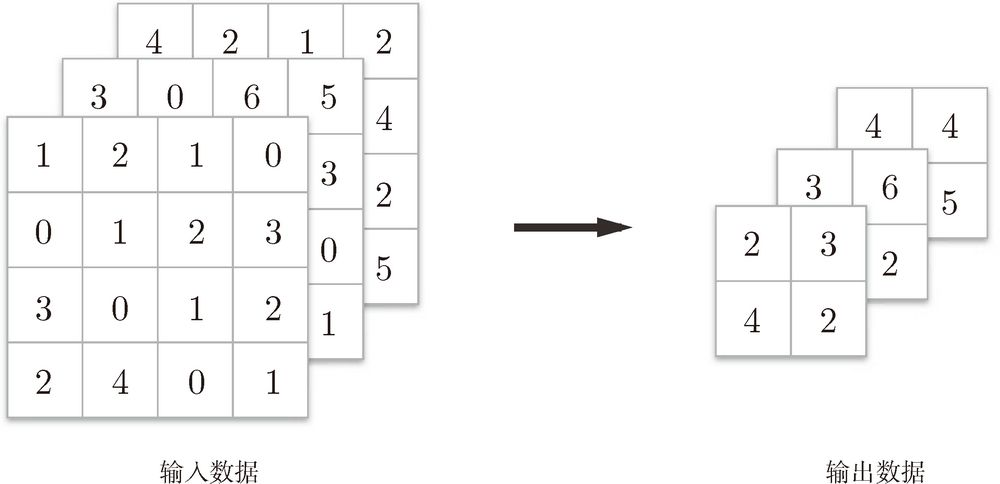
\includegraphics[width=\textwidth]{Figures/The number of channels in pooling remains unchanged.png}
        \caption{The number of channels in pooling remains unchanged}
        \label{fig7-15a}
    \end{subfigure}
    \hfill
    \begin{subfigure}{.45\textwidth}
        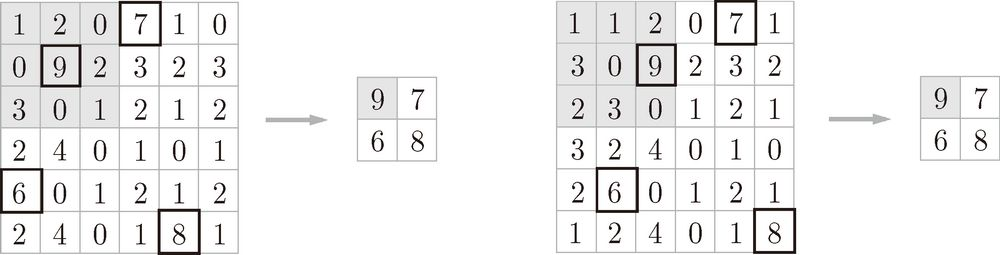
\includegraphics[width=\textwidth]{Figures/Robust to small position changes.png}
        \caption{Robust to small position changes}
        \label{fig7-15b}
    \end{subfigure}
    \caption{Features of the pooling layer}
    \label{fig7-15}
\end{figure}
\section{卷积层和池化层的实现}
\subsection{4维数组}
所谓4维数据,比如
数据的形状是$(10, 1, 28, 28)$,则它对应10个高为28、长为28、通道为1的数
据。
\subsection{基于im2col的展开}
NumPy中存在使用 for语句后处理变慢的缺点(NumPy 中,访问元素时最好不要用 for语句)。

im2col是一个函数,将输入数据展开以适合滤波器(权重)。如 \autoref{fig7-16a} 所示,
对3维的输入数据应用 im2col后,数据转换为2维矩阵(正确地讲,是把包含
批数量的4维数据转换成了2维数据)。

im2col会把输入数据展开以适合滤波器(权重)。具体地说,如 \autoref{fig7-16b} 所示,
对于输入数据,将应用滤波器的区域(3维方块)横向展开为1列。im2col会
在所有应用滤波器的地方进行这个展开处理。

\begin{figure}
    \centering
    \begin{subfigure}{.45\textwidth}
        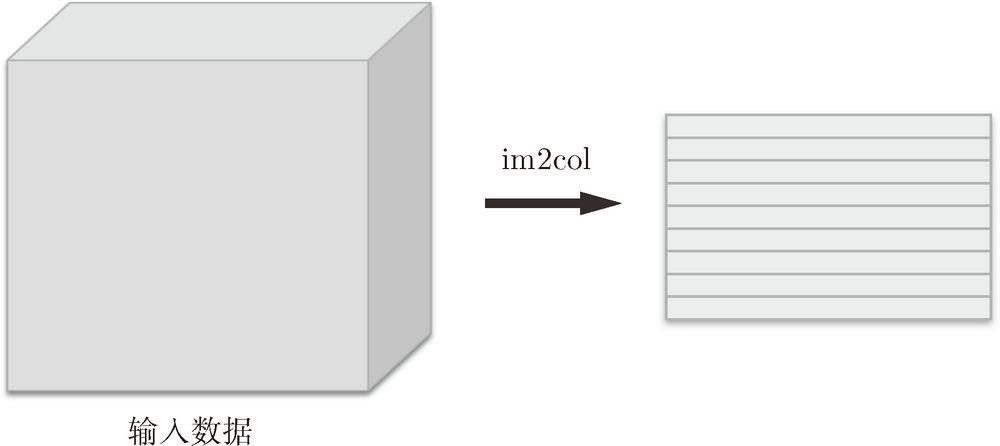
\includegraphics[width=\textwidth]{Figures/Schematic diagram of im2col.png}
        \caption{Schematic diagram of im2col}
        \label{fig7-16a}
    \end{subfigure}
    \hfill
    \begin{subfigure}{.45\textwidth}
        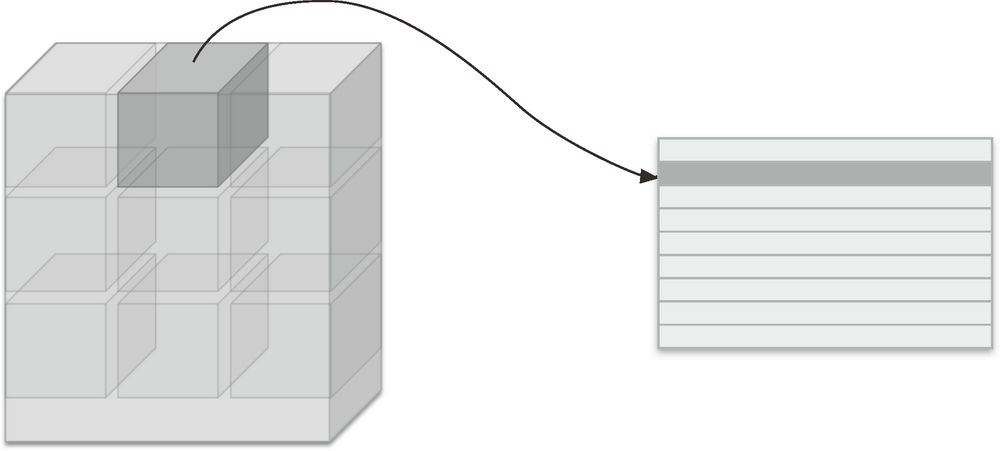
\includegraphics[width=\textwidth]{Figures/Expand the filter's application area sequentially from the beginning to 1 column horizontally.png}
        \caption{Robust to small position changes}
        \label{fig7-16b}
    \end{subfigure}
    \caption{function im2col}
    \label{fig7-16}
\end{figure}

在 \autoref{fig7-16b} 中,为了便于观察,将步幅设置得很大,以使滤波器的应用区
域不重叠。而在实际的卷积运算中,滤波器的应用区域几乎都是重叠的。在
滤波器的应用区域重叠的情况下,使用 im2col展开后,展开后的元素个数会
多于原方块的元素个数。因此,使用 im2col的实现存在比普通的实现消耗更
多内存的缺点。但是,汇总成一个大的矩阵进行计算,对计算机的计算颇有
益处。比如,在矩阵计算的库(线性代数库)等中,矩阵计算的实现已被高
度最优化,可以高速地进行大矩阵的乘法运算。因此,通过归结到矩阵计算
上,可以有效地利用线性代数库。

\begin{tcolorbox}
    im2col这个名称是“image to column”的缩写,翻译过来就是“从
    图像到矩阵”的意思。Caffe、Chainer 等深度学习框架中有名为
    im2col的函数,并且在卷积层的实现中,都使用了 im2col。
\end{tcolorbox}

使用 im2col展开输入数据后,之后就只需将卷积层的滤波器(权重)纵
向展开为1列,并计算2个矩阵的乘积即可(参照 \autoref{Details of filter processing for convolution operations})。

如 \autoref{Details of filter processing for convolution operations} 所示,基于 im2col方式的输出结果是2维矩阵。因为CNN中
数据会保存为4维数组,所以要将2维输出数据转换为合适的形状。

\figures{Details of filter processing for convolution operations}

\subsection{卷积层的实现}